\documentclass{mipt-thesis-bs}
% Следующие две строки нужны только для biblatex. Для inline-библиографии их следует убрать.
\usepackage{mipt-thesis-biblatex}
\usepackage[justification=centering]{caption}
\usepackage{glossaries}
\usepackage{url}
\usepackage{pdfpages}
\usepackage{hyperref}
\usepackage[title]{appendix}
\addbibresource{ref.bib}



\title{Применение генеративного моделирования как инструмента постановки естественнонаучной задачи педагогической направленности}
\author{Машалов Никита}
\supervisor{Щербаков Дмитрий}
%\referee{Петров Д.\,Е.}       % требуется только для mipt-thesis-ms
\groupnum{БО2-886}
\faculty{Физтех-школа физики и исследований им. Ландау}
\department{Кафедра инновационной педагогики}


\begin{document}
% Абстракт

\tableofcontents

\pagebreak

Анализ естественного языка это межпредметная дисциплина.

\begin{figure}[h]
    \centering
    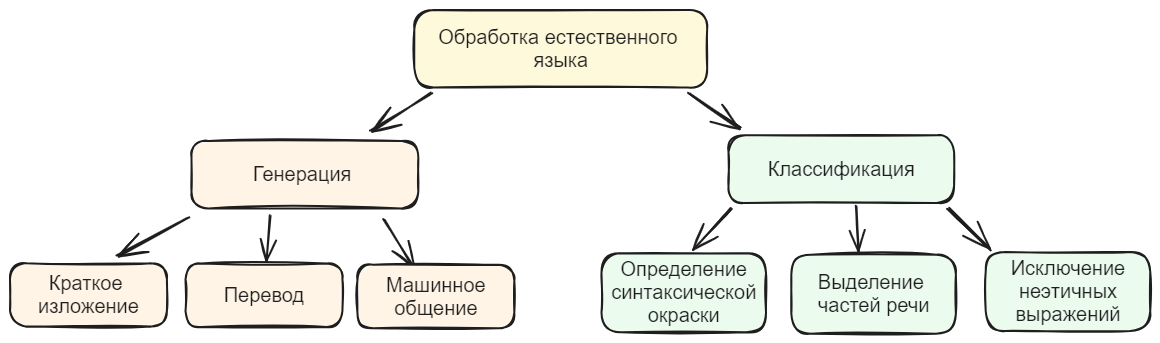
\includegraphics[width=0.5\textwidth]{assets/ml/nlp/taxonomy.excalidraw.png}
    \caption{Таксономия современных подходов обработки естественного языка}
    \label{llm_taxonomy}
\end{figure}

Формальные языки широко используются в математике, логике, лингвистике и компьютерных науках. 
В программировании, например, формальные языки включают языки программирования и описания данных, 
где синтаксис строго определён для обеспечения корректности и предсказуемости выполнения программ.

особенно важным для развития генеративного моделирования.
В областях обработки естественного языка стала популярна аналитическая форма механизма внимания \cite{vaswani2017attention},
приведшая к созданию больших лингвистических моделей \cite{radford2019language}, имеющих важное практическое применение.


\chapter{Математические основы машинного обучения}
Анализ естественного языка это межпредметная дисциплина.

\begin{figure}[h]
    \centering
    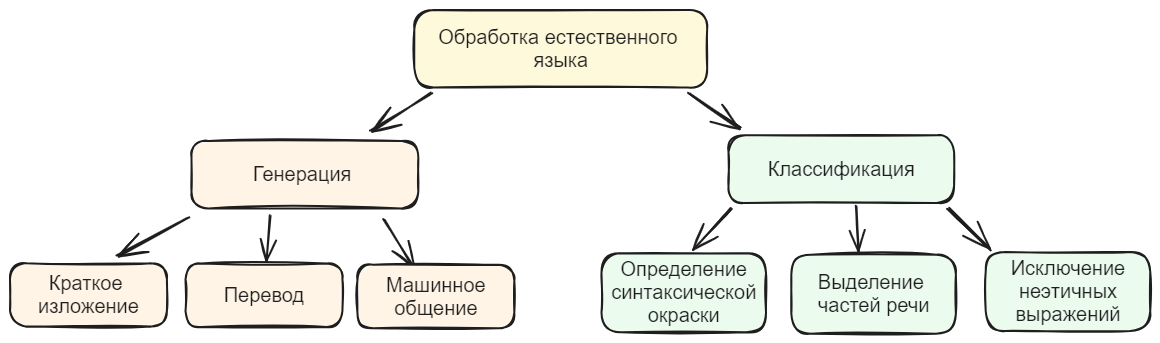
\includegraphics[width=0.5\textwidth]{assets/ml/nlp/taxonomy.excalidraw.png}
    \caption{Таксономия современных подходов обработки естественного языка}
    \label{llm_taxonomy}
\end{figure}

Формальные языки широко используются в математике, логике, лингвистике и компьютерных науках. 
В программировании, например, формальные языки включают языки программирования и описания данных, 
где синтаксис строго определён для обеспечения корректности и предсказуемости выполнения программ.

особенно важным для развития генеративного моделирования.
В областях обработки естественного языка стала популярна аналитическая форма механизма внимания \cite{vaswani2017attention},
приведшая к созданию больших лингвистических моделей \cite{radford2019language}, имеющих важное практическое применение.



\subsection{Оптимизация графа}

Задача оптимального транспорта (Optimal Transport)\cite{villani2009optimal} является одной из ключевых  
в области теории вероятностей и машинного обучения.
Она представляет собой проблему определения оптимального способа перемещения вероятностной массы из одной 
распределенной системы в другую с минимальными затратами или стоимостью. Формально задача состоит в составлении 
транспортного плана \( T: \mathcal{X} \rightarrow \mathcal{Y} \), 
который переводит распределение \( \mu \subset \mathcal{X}\) в распределение \( \nu \subset \mathcal{Y} \), минимизируя некоторую функцию стоимости. 
Функция стоимости $c: \mathcal{X} \times \mathcal{Y} \rightarrow \mathbb{R}$ обычно является мерой сходства между элементами из \( \mathcal{X} \) и \( \mathcal{Y} \), 
такой как квадрат расстояния. 

\textit{Определение} (Монже): \textbf{Оптимальный транспорт} по Монже вводится путем рассмотрения вероятностных 
распределений \( \mu \) и \( \nu \) на метрических пространствах \( \mathcal{X} \) и \( \mathcal{Y} \):
\begin{equation}
    \inf_{\gamma \in \Pi(\mu, \nu)} \int_{\mathcal{X} \times \mathcal{Y}} c(x,y) \, d\gamma(x,y),
\end{equation}
где \( \Pi(\mu, \nu) \) обозначает множество всех возможных совместных распределений 
\( \gamma \) на \( \mathcal{X} \times \mathcal{Y} \) с фиксированными маргинальными
распределениями \( \mu \) и \( \nu \), а \( c(x,y) \) — функция стоимости перевозки массы из \( x \) в \( y \).

\textit{Определение} (Канторович): \textbf{Оптимальный транспорт} по Канторовичу  вводится через потенциал $\phi$, 
который минимизирует функционал стоимости:
\begin{equation}
    \inf_{\phi} \left( \int_{\mathcal{X}} \phi(x) \, d\mu(x) + \int_{\mathcal{Y}} \psi(y) \, d\nu(y) \right),
\end{equation}
где \( \psi \) — обратная функция к \( \phi \). Таким образом, 
отображение \( T: \mathcal{X} \rightarrow \mathcal{Y} \) вытекает из градиента потенциала.

Заметим, что постановка Канторовича обобщает постановку Монже\ref{monge_vs_kantarovich}. В отличие от постановки Монже 
оптимальный транспорт по Канторовичу допускает распределение вероятностной массы в непрерывном случае.

\begin{figure}[h]
    \centering
    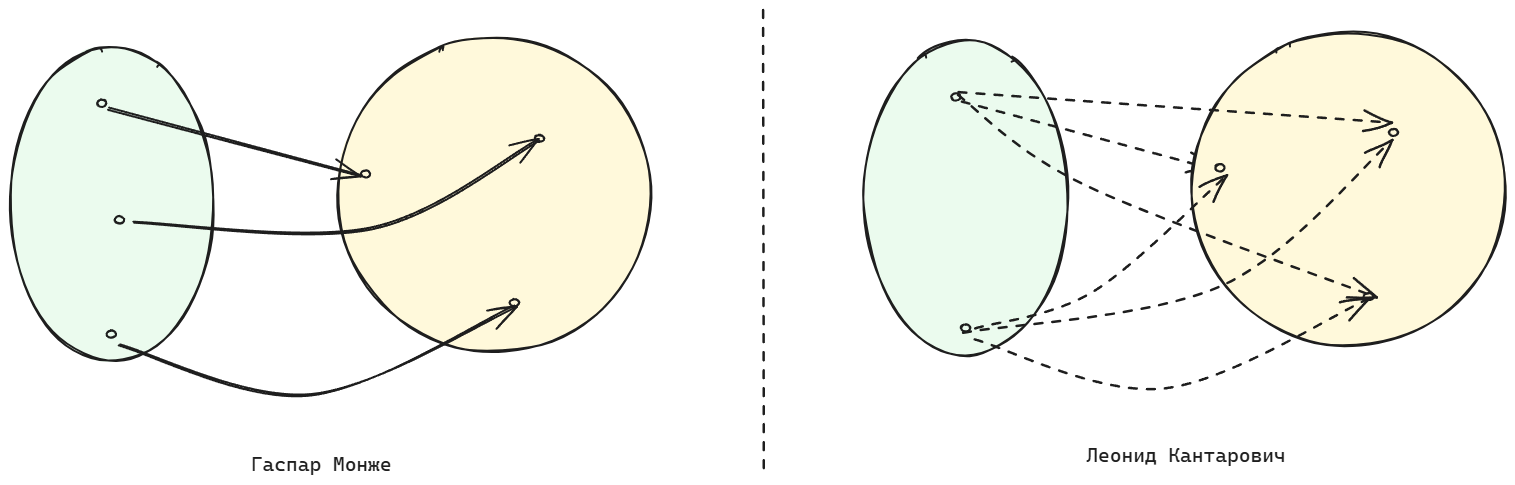
\includegraphics[width=0.7\textwidth]{assets/math/transport/optimal_transport.excalidraw.png}
    \caption{Различие в подходе по Монже и Кантаровичу. В постановке Канторовича задача релаксирует до 
    непрерывного распределения}
    \label{monge_vs_kantarovich}
\end{figure}

Итоговая стоимость оптимального транспортного плана называется метрикой Вассерштейна.

\textit{Определение:} Пусть \((X, d)\) --- метрическое пространство и \(P(X)\) --- множество всех вероятностных мер на \(X\). 
Для двух вероятностных мер \(\mu\) и \(\nu\) на \(X\) \textbf{метрика Вассерштейна} порядка \(p\), где \(p \geq 1\), определяется как:
\begin{equation}
    W_p(\mu, \nu) = \left( \inf_{\gamma \in \Gamma(\mu, \nu)} \int_{X \times X} d(x, y)^p \, d\gamma(x, y) \right)^{1/p},
\end{equation}
где \(\Gamma(\mu, \nu)\) — множество всех сопряжённых мер \(\gamma\) на \(X \times X\) с маргиналами \(\mu\) и \(\nu\).

Метрика имеет практическое применение для задач физики, биологии и машинного обучения, поскольку задает 
дифференцируемую разность между распределениями.

\textit{Определение:} \textbf{Метрическая производная} кривой $\rho_t,t \in [0,T]$ в вероятностном 
пространстве $\mathcal{P}_2(\mathbb{R}^N)$ запишется как:
\begin{equation}
    |\rho_t'| = \lim_{dt \rightarrow 0} \frac{\mathcal{W}_2(\rho_t, \rho_{t+dt})}{dt}
\end{equation}

Метод оптимального транспорта также активно применяется для анализа стохастических процессов. Базовой моделью, 
описывающей стохастическое движение с смещением, является процесс Ланжевена.

\textit{Определение:} Процесс Ланжевена называется случайнный процесс вида
\begin{equation}
    d X_t = - \nabla \Phi(x) dt + \sqrt{2 \beta^{-1}} d W_t,
\end{equation}
где $\Phi(X)$ --- потенциал задающий снос частицы, $\beta$ - масштаб блуждания и  $d W_t$ - процесс Винера.

\begin{figure}[h]
    \centering
    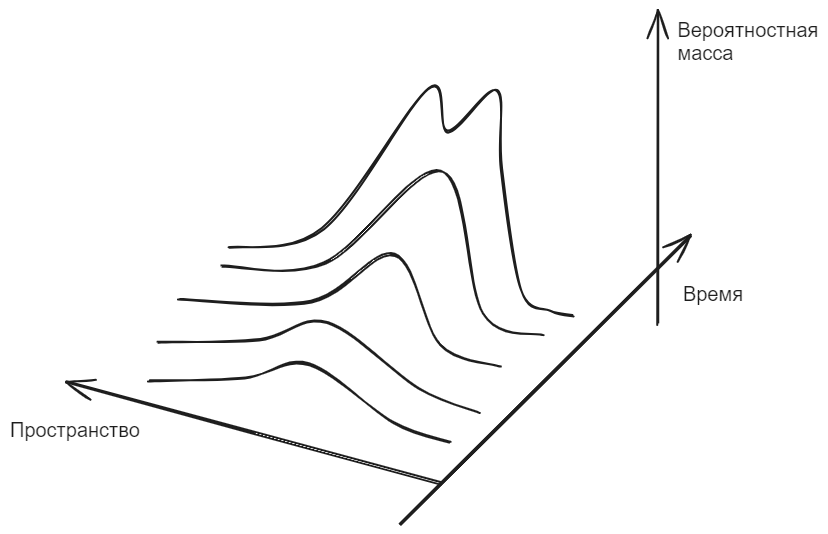
\includegraphics[width=0.5\textwidth]{assets/math/transport/fokker-plank.excalidraw.png}
    \caption{Эволюция вероятностной массы в уравнение Ланжевена}
    \label{opt_transport}
\end{figure}

Стохастическое усреднение процесса Ланжевена можно описать с помощью уравнения Колмогорова-Фоккера-Планка, 
задающего эволюцию вероятностной массы в дифференциальной форме  $\rho_t(x)$:
\begin{equation}
    \frac{\partial \rho_t}{\partial t} = \text{div}(\nabla \Phi(x) \rho_t) + \beta^{-1} \Delta \rho_t.
\end{equation}

Для естественной работы в энергетических постановках водится функционал, задающий коэффициента сноса с потенциалом $\Phi$.
Таким образом, исходное уравнение можно переписать в вариационной постановке \ref{variation_fp}.

\textit{Определение:} \textbf{Функционал Фоккера-Планка} для распределения $\rho$ записывается как: 
\begin{equation}
    \mathcal{F}_{FP}(\rho) = \int  \Phi(x) d\rho(x) + \beta^{-1} \int \log \rho(x) d \rho(x).
\end{equation}
\begin{figure}[h]
    \centering
    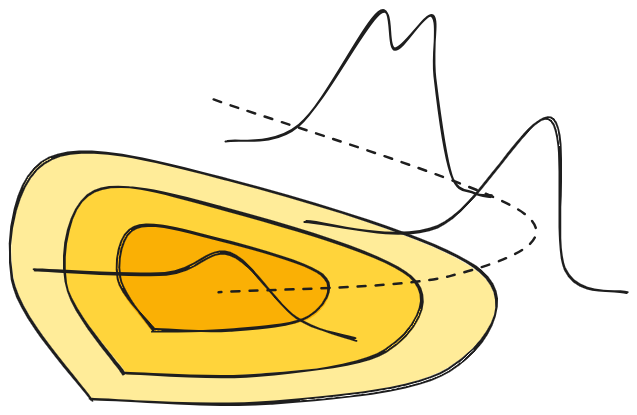
\includegraphics[width=0.5\textwidth]{assets/math/transport/functional.excalidraw.png}
    \caption{Визуализация постановки уравнения Фоккера-Планка в вариационной форме}
    \label{variation_fp}
\end{figure}
Научная группа Йордана-Кинана-Отто в работе \cite{jordan1998variational} показала, что маргинальные вероятностные
меры процесса Ланжевена подчиняются уравнению градиентного потока Вассерштейна относительно функционала Фоккера-Планка.

\textit{Определение:}  \textbf{Схема Йордана-Кинана-Отто} задает правило обновления уравнения вероятности в виде
минимизации функционала энергии и расстояния:
\begin{equation}
    \rho^{n+1} = \underset{\rho}{\operatorname{argmin}} \left( \frac{1}{2\tau} W_2^2(\rho, \rho^n) + \mathcal{F}(\rho) \right),
\end{equation}
где:\begin{itemize}
    \item \(\tau > 0\) --- шаг по времени;
    \item \(W_2(\rho, \rho^n)\) --- метрика Вассерштейна 2-го порядка между плотностями \(\rho\) и \(\rho^n\);
    \item  \(\mathcal{F}(\rho)\) --- функционал свободной энергии, который может включать в себя энтропийный член и 
    потенциальную энергию системы.
\end{itemize}
Функционал свободной энергии\(\mathcal{F}(\rho)\) задается в виде:
\begin{equation}
    \mathcal{F}(\rho) = \int_V f(\rho(x)) \, dx + \int_V V(x) \rho(x) \, dx,
\end{equation}
где \(f(\rho)\) — внутренний энергетический член, зависящий от плотности, а \(V(x)\) — внешний потенциал.




\chapter{Методы машинного обучения}
Анализ естественного языка это межпредметная дисциплина.

\begin{figure}[h]
    \centering
    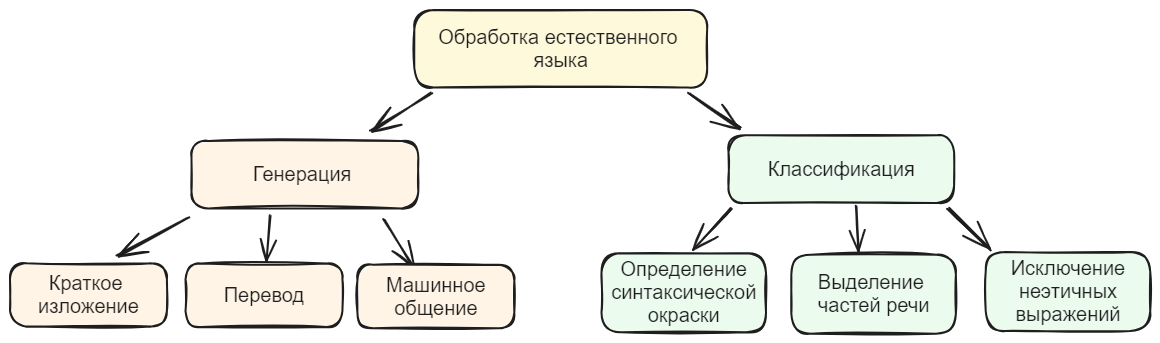
\includegraphics[width=0.5\textwidth]{assets/ml/nlp/taxonomy.excalidraw.png}
    \caption{Таксономия современных подходов обработки естественного языка}
    \label{llm_taxonomy}
\end{figure}

Формальные языки широко используются в математике, логике, лингвистике и компьютерных науках. 
В программировании, например, формальные языки включают языки программирования и описания данных, 
где синтаксис строго определён для обеспечения корректности и предсказуемости выполнения программ.

особенно важным для развития генеративного моделирования.
В областях обработки естественного языка стала популярна аналитическая форма механизма внимания \cite{vaswani2017attention},
приведшая к созданию больших лингвистических моделей \cite{radford2019language}, имеющих важное практическое применение.



\subsection{Оптимизация графа}

Задача оптимального транспорта (Optimal Transport)\cite{villani2009optimal} является одной из ключевых  
в области теории вероятностей и машинного обучения.
Она представляет собой проблему определения оптимального способа перемещения вероятностной массы из одной 
распределенной системы в другую с минимальными затратами или стоимостью. Формально задача состоит в составлении 
транспортного плана \( T: \mathcal{X} \rightarrow \mathcal{Y} \), 
который переводит распределение \( \mu \subset \mathcal{X}\) в распределение \( \nu \subset \mathcal{Y} \), минимизируя некоторую функцию стоимости. 
Функция стоимости $c: \mathcal{X} \times \mathcal{Y} \rightarrow \mathbb{R}$ обычно является мерой сходства между элементами из \( \mathcal{X} \) и \( \mathcal{Y} \), 
такой как квадрат расстояния. 

\textit{Определение} (Монже): \textbf{Оптимальный транспорт} по Монже вводится путем рассмотрения вероятностных 
распределений \( \mu \) и \( \nu \) на метрических пространствах \( \mathcal{X} \) и \( \mathcal{Y} \):
\begin{equation}
    \inf_{\gamma \in \Pi(\mu, \nu)} \int_{\mathcal{X} \times \mathcal{Y}} c(x,y) \, d\gamma(x,y),
\end{equation}
где \( \Pi(\mu, \nu) \) обозначает множество всех возможных совместных распределений 
\( \gamma \) на \( \mathcal{X} \times \mathcal{Y} \) с фиксированными маргинальными
распределениями \( \mu \) и \( \nu \), а \( c(x,y) \) — функция стоимости перевозки массы из \( x \) в \( y \).

\textit{Определение} (Канторович): \textbf{Оптимальный транспорт} по Канторовичу  вводится через потенциал $\phi$, 
который минимизирует функционал стоимости:
\begin{equation}
    \inf_{\phi} \left( \int_{\mathcal{X}} \phi(x) \, d\mu(x) + \int_{\mathcal{Y}} \psi(y) \, d\nu(y) \right),
\end{equation}
где \( \psi \) — обратная функция к \( \phi \). Таким образом, 
отображение \( T: \mathcal{X} \rightarrow \mathcal{Y} \) вытекает из градиента потенциала.

Заметим, что постановка Канторовича обобщает постановку Монже\ref{monge_vs_kantarovich}. В отличие от постановки Монже 
оптимальный транспорт по Канторовичу допускает распределение вероятностной массы в непрерывном случае.

\begin{figure}[h]
    \centering
    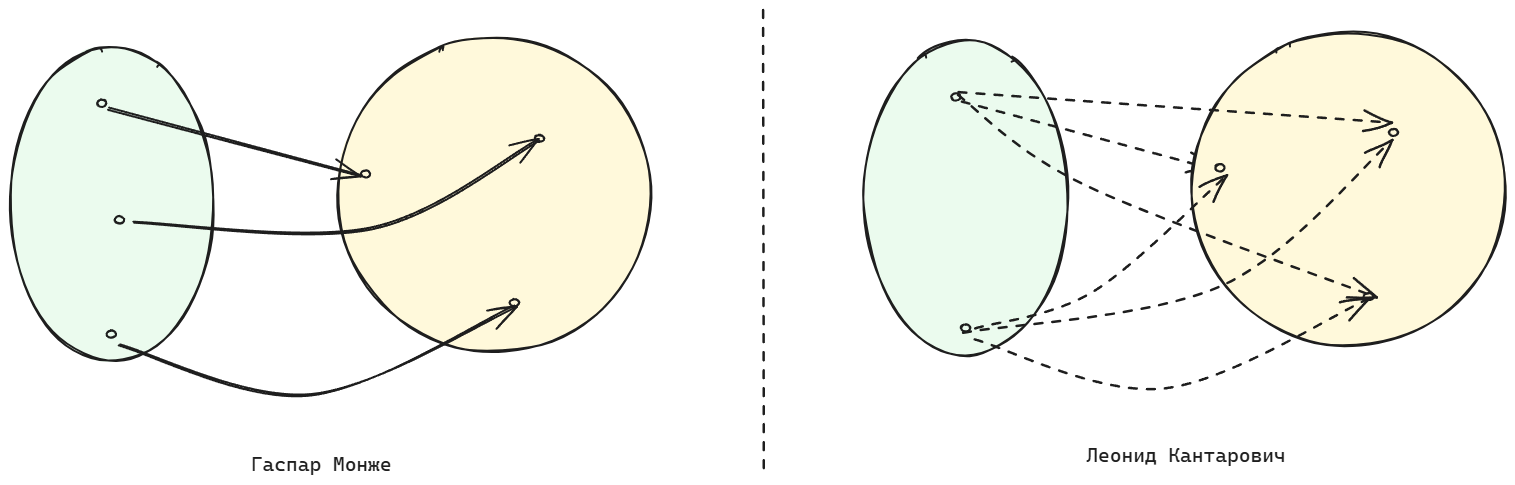
\includegraphics[width=0.7\textwidth]{assets/math/transport/optimal_transport.excalidraw.png}
    \caption{Различие в подходе по Монже и Кантаровичу. В постановке Канторовича задача релаксирует до 
    непрерывного распределения}
    \label{monge_vs_kantarovich}
\end{figure}

Итоговая стоимость оптимального транспортного плана называется метрикой Вассерштейна.

\textit{Определение:} Пусть \((X, d)\) --- метрическое пространство и \(P(X)\) --- множество всех вероятностных мер на \(X\). 
Для двух вероятностных мер \(\mu\) и \(\nu\) на \(X\) \textbf{метрика Вассерштейна} порядка \(p\), где \(p \geq 1\), определяется как:
\begin{equation}
    W_p(\mu, \nu) = \left( \inf_{\gamma \in \Gamma(\mu, \nu)} \int_{X \times X} d(x, y)^p \, d\gamma(x, y) \right)^{1/p},
\end{equation}
где \(\Gamma(\mu, \nu)\) — множество всех сопряжённых мер \(\gamma\) на \(X \times X\) с маргиналами \(\mu\) и \(\nu\).

Метрика имеет практическое применение для задач физики, биологии и машинного обучения, поскольку задает 
дифференцируемую разность между распределениями.

\textit{Определение:} \textbf{Метрическая производная} кривой $\rho_t,t \in [0,T]$ в вероятностном 
пространстве $\mathcal{P}_2(\mathbb{R}^N)$ запишется как:
\begin{equation}
    |\rho_t'| = \lim_{dt \rightarrow 0} \frac{\mathcal{W}_2(\rho_t, \rho_{t+dt})}{dt}
\end{equation}

Метод оптимального транспорта также активно применяется для анализа стохастических процессов. Базовой моделью, 
описывающей стохастическое движение с смещением, является процесс Ланжевена.

\textit{Определение:} Процесс Ланжевена называется случайнный процесс вида
\begin{equation}
    d X_t = - \nabla \Phi(x) dt + \sqrt{2 \beta^{-1}} d W_t,
\end{equation}
где $\Phi(X)$ --- потенциал задающий снос частицы, $\beta$ - масштаб блуждания и  $d W_t$ - процесс Винера.

\begin{figure}[h]
    \centering
    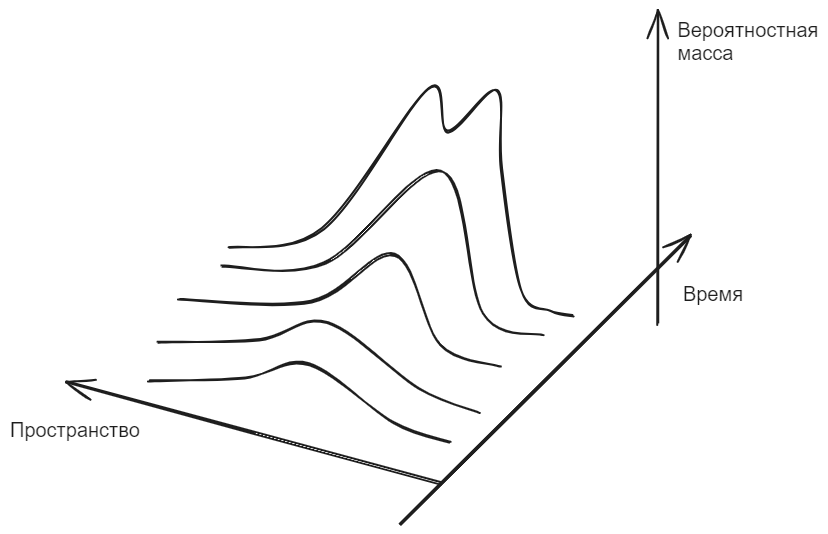
\includegraphics[width=0.5\textwidth]{assets/math/transport/fokker-plank.excalidraw.png}
    \caption{Эволюция вероятностной массы в уравнение Ланжевена}
    \label{opt_transport}
\end{figure}

Стохастическое усреднение процесса Ланжевена можно описать с помощью уравнения Колмогорова-Фоккера-Планка, 
задающего эволюцию вероятностной массы в дифференциальной форме  $\rho_t(x)$:
\begin{equation}
    \frac{\partial \rho_t}{\partial t} = \text{div}(\nabla \Phi(x) \rho_t) + \beta^{-1} \Delta \rho_t.
\end{equation}

Для естественной работы в энергетических постановках водится функционал, задающий коэффициента сноса с потенциалом $\Phi$.
Таким образом, исходное уравнение можно переписать в вариационной постановке \ref{variation_fp}.

\textit{Определение:} \textbf{Функционал Фоккера-Планка} для распределения $\rho$ записывается как: 
\begin{equation}
    \mathcal{F}_{FP}(\rho) = \int  \Phi(x) d\rho(x) + \beta^{-1} \int \log \rho(x) d \rho(x).
\end{equation}
\begin{figure}[h]
    \centering
    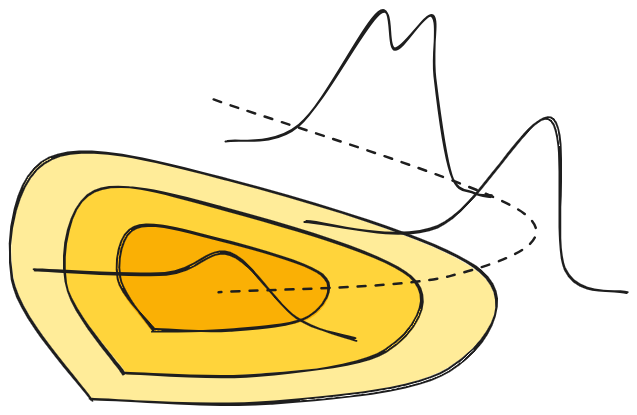
\includegraphics[width=0.5\textwidth]{assets/math/transport/functional.excalidraw.png}
    \caption{Визуализация постановки уравнения Фоккера-Планка в вариационной форме}
    \label{variation_fp}
\end{figure}
Научная группа Йордана-Кинана-Отто в работе \cite{jordan1998variational} показала, что маргинальные вероятностные
меры процесса Ланжевена подчиняются уравнению градиентного потока Вассерштейна относительно функционала Фоккера-Планка.

\textit{Определение:}  \textbf{Схема Йордана-Кинана-Отто} задает правило обновления уравнения вероятности в виде
минимизации функционала энергии и расстояния:
\begin{equation}
    \rho^{n+1} = \underset{\rho}{\operatorname{argmin}} \left( \frac{1}{2\tau} W_2^2(\rho, \rho^n) + \mathcal{F}(\rho) \right),
\end{equation}
где:\begin{itemize}
    \item \(\tau > 0\) --- шаг по времени;
    \item \(W_2(\rho, \rho^n)\) --- метрика Вассерштейна 2-го порядка между плотностями \(\rho\) и \(\rho^n\);
    \item  \(\mathcal{F}(\rho)\) --- функционал свободной энергии, который может включать в себя энтропийный член и 
    потенциальную энергию системы.
\end{itemize}
Функционал свободной энергии\(\mathcal{F}(\rho)\) задается в виде:
\begin{equation}
    \mathcal{F}(\rho) = \int_V f(\rho(x)) \, dx + \int_V V(x) \rho(x) \, dx,
\end{equation}
где \(f(\rho)\) — внутренний энергетический член, зависящий от плотности, а \(V(x)\) — внешний потенциал.




\chapter{Математические методы в педагогике}
Анализ естественного языка это межпредметная дисциплина.

\begin{figure}[h]
    \centering
    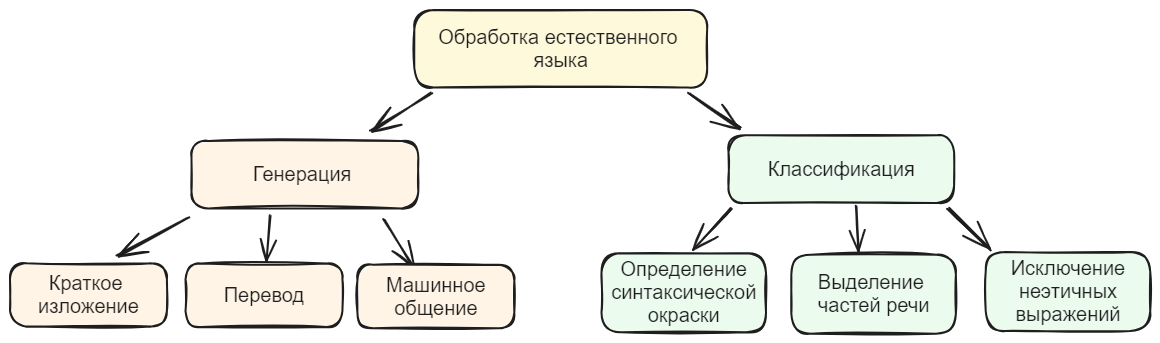
\includegraphics[width=0.5\textwidth]{assets/ml/nlp/taxonomy.excalidraw.png}
    \caption{Таксономия современных подходов обработки естественного языка}
    \label{llm_taxonomy}
\end{figure}

Формальные языки широко используются в математике, логике, лингвистике и компьютерных науках. 
В программировании, например, формальные языки включают языки программирования и описания данных, 
где синтаксис строго определён для обеспечения корректности и предсказуемости выполнения программ.

особенно важным для развития генеративного моделирования.
В областях обработки естественного языка стала популярна аналитическая форма механизма внимания \cite{vaswani2017attention},
приведшая к созданию больших лингвистических моделей \cite{radford2019language}, имеющих важное практическое применение.



\subsection{Оптимизация графа}

Задача оптимального транспорта (Optimal Transport)\cite{villani2009optimal} является одной из ключевых  
в области теории вероятностей и машинного обучения.
Она представляет собой проблему определения оптимального способа перемещения вероятностной массы из одной 
распределенной системы в другую с минимальными затратами или стоимостью. Формально задача состоит в составлении 
транспортного плана \( T: \mathcal{X} \rightarrow \mathcal{Y} \), 
который переводит распределение \( \mu \subset \mathcal{X}\) в распределение \( \nu \subset \mathcal{Y} \), минимизируя некоторую функцию стоимости. 
Функция стоимости $c: \mathcal{X} \times \mathcal{Y} \rightarrow \mathbb{R}$ обычно является мерой сходства между элементами из \( \mathcal{X} \) и \( \mathcal{Y} \), 
такой как квадрат расстояния. 

\textit{Определение} (Монже): \textbf{Оптимальный транспорт} по Монже вводится путем рассмотрения вероятностных 
распределений \( \mu \) и \( \nu \) на метрических пространствах \( \mathcal{X} \) и \( \mathcal{Y} \):
\begin{equation}
    \inf_{\gamma \in \Pi(\mu, \nu)} \int_{\mathcal{X} \times \mathcal{Y}} c(x,y) \, d\gamma(x,y),
\end{equation}
где \( \Pi(\mu, \nu) \) обозначает множество всех возможных совместных распределений 
\( \gamma \) на \( \mathcal{X} \times \mathcal{Y} \) с фиксированными маргинальными
распределениями \( \mu \) и \( \nu \), а \( c(x,y) \) — функция стоимости перевозки массы из \( x \) в \( y \).

\textit{Определение} (Канторович): \textbf{Оптимальный транспорт} по Канторовичу  вводится через потенциал $\phi$, 
который минимизирует функционал стоимости:
\begin{equation}
    \inf_{\phi} \left( \int_{\mathcal{X}} \phi(x) \, d\mu(x) + \int_{\mathcal{Y}} \psi(y) \, d\nu(y) \right),
\end{equation}
где \( \psi \) — обратная функция к \( \phi \). Таким образом, 
отображение \( T: \mathcal{X} \rightarrow \mathcal{Y} \) вытекает из градиента потенциала.

Заметим, что постановка Канторовича обобщает постановку Монже\ref{monge_vs_kantarovich}. В отличие от постановки Монже 
оптимальный транспорт по Канторовичу допускает распределение вероятностной массы в непрерывном случае.

\begin{figure}[h]
    \centering
    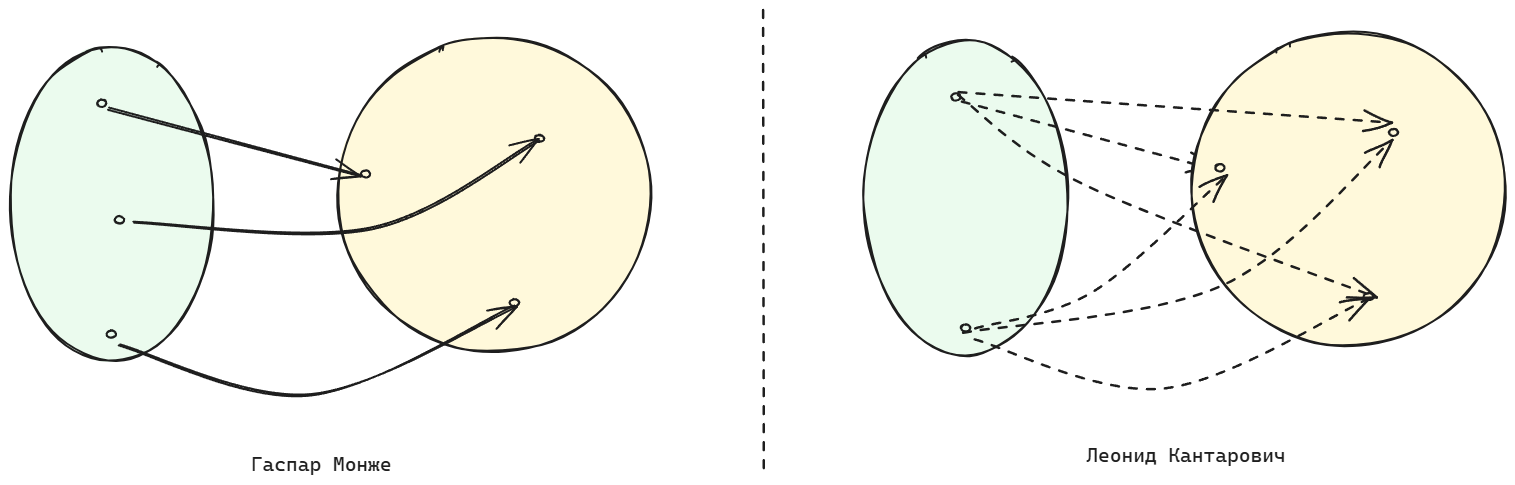
\includegraphics[width=0.7\textwidth]{assets/math/transport/optimal_transport.excalidraw.png}
    \caption{Различие в подходе по Монже и Кантаровичу. В постановке Канторовича задача релаксирует до 
    непрерывного распределения}
    \label{monge_vs_kantarovich}
\end{figure}

Итоговая стоимость оптимального транспортного плана называется метрикой Вассерштейна.

\textit{Определение:} Пусть \((X, d)\) --- метрическое пространство и \(P(X)\) --- множество всех вероятностных мер на \(X\). 
Для двух вероятностных мер \(\mu\) и \(\nu\) на \(X\) \textbf{метрика Вассерштейна} порядка \(p\), где \(p \geq 1\), определяется как:
\begin{equation}
    W_p(\mu, \nu) = \left( \inf_{\gamma \in \Gamma(\mu, \nu)} \int_{X \times X} d(x, y)^p \, d\gamma(x, y) \right)^{1/p},
\end{equation}
где \(\Gamma(\mu, \nu)\) — множество всех сопряжённых мер \(\gamma\) на \(X \times X\) с маргиналами \(\mu\) и \(\nu\).

Метрика имеет практическое применение для задач физики, биологии и машинного обучения, поскольку задает 
дифференцируемую разность между распределениями.

\textit{Определение:} \textbf{Метрическая производная} кривой $\rho_t,t \in [0,T]$ в вероятностном 
пространстве $\mathcal{P}_2(\mathbb{R}^N)$ запишется как:
\begin{equation}
    |\rho_t'| = \lim_{dt \rightarrow 0} \frac{\mathcal{W}_2(\rho_t, \rho_{t+dt})}{dt}
\end{equation}

Метод оптимального транспорта также активно применяется для анализа стохастических процессов. Базовой моделью, 
описывающей стохастическое движение с смещением, является процесс Ланжевена.

\textit{Определение:} Процесс Ланжевена называется случайнный процесс вида
\begin{equation}
    d X_t = - \nabla \Phi(x) dt + \sqrt{2 \beta^{-1}} d W_t,
\end{equation}
где $\Phi(X)$ --- потенциал задающий снос частицы, $\beta$ - масштаб блуждания и  $d W_t$ - процесс Винера.

\begin{figure}[h]
    \centering
    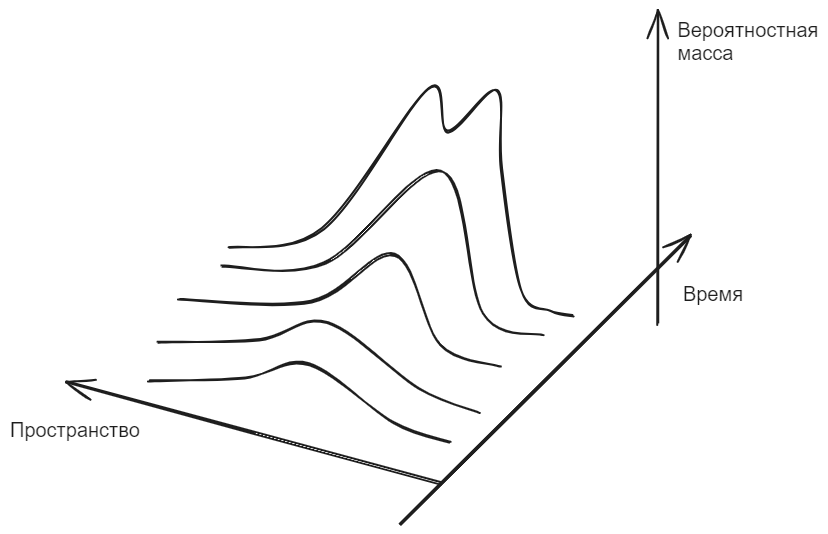
\includegraphics[width=0.5\textwidth]{assets/math/transport/fokker-plank.excalidraw.png}
    \caption{Эволюция вероятностной массы в уравнение Ланжевена}
    \label{opt_transport}
\end{figure}

Стохастическое усреднение процесса Ланжевена можно описать с помощью уравнения Колмогорова-Фоккера-Планка, 
задающего эволюцию вероятностной массы в дифференциальной форме  $\rho_t(x)$:
\begin{equation}
    \frac{\partial \rho_t}{\partial t} = \text{div}(\nabla \Phi(x) \rho_t) + \beta^{-1} \Delta \rho_t.
\end{equation}

Для естественной работы в энергетических постановках водится функционал, задающий коэффициента сноса с потенциалом $\Phi$.
Таким образом, исходное уравнение можно переписать в вариационной постановке \ref{variation_fp}.

\textit{Определение:} \textbf{Функционал Фоккера-Планка} для распределения $\rho$ записывается как: 
\begin{equation}
    \mathcal{F}_{FP}(\rho) = \int  \Phi(x) d\rho(x) + \beta^{-1} \int \log \rho(x) d \rho(x).
\end{equation}
\begin{figure}[h]
    \centering
    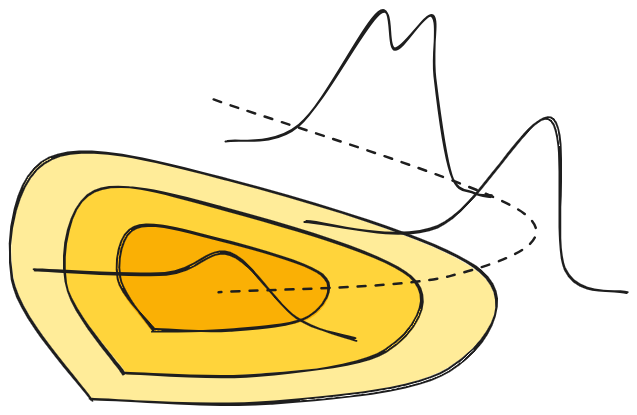
\includegraphics[width=0.5\textwidth]{assets/math/transport/functional.excalidraw.png}
    \caption{Визуализация постановки уравнения Фоккера-Планка в вариационной форме}
    \label{variation_fp}
\end{figure}
Научная группа Йордана-Кинана-Отто в работе \cite{jordan1998variational} показала, что маргинальные вероятностные
меры процесса Ланжевена подчиняются уравнению градиентного потока Вассерштейна относительно функционала Фоккера-Планка.

\textit{Определение:}  \textbf{Схема Йордана-Кинана-Отто} задает правило обновления уравнения вероятности в виде
минимизации функционала энергии и расстояния:
\begin{equation}
    \rho^{n+1} = \underset{\rho}{\operatorname{argmin}} \left( \frac{1}{2\tau} W_2^2(\rho, \rho^n) + \mathcal{F}(\rho) \right),
\end{equation}
где:\begin{itemize}
    \item \(\tau > 0\) --- шаг по времени;
    \item \(W_2(\rho, \rho^n)\) --- метрика Вассерштейна 2-го порядка между плотностями \(\rho\) и \(\rho^n\);
    \item  \(\mathcal{F}(\rho)\) --- функционал свободной энергии, который может включать в себя энтропийный член и 
    потенциальную энергию системы.
\end{itemize}
Функционал свободной энергии\(\mathcal{F}(\rho)\) задается в виде:
\begin{equation}
    \mathcal{F}(\rho) = \int_V f(\rho(x)) \, dx + \int_V V(x) \rho(x) \, dx,
\end{equation}
где \(f(\rho)\) — внутренний энергетический член, зависящий от плотности, а \(V(x)\) — внешний потенциал.




\chapter{Описание работы}
Анализ естественного языка это межпредметная дисциплина.

\begin{figure}[h]
    \centering
    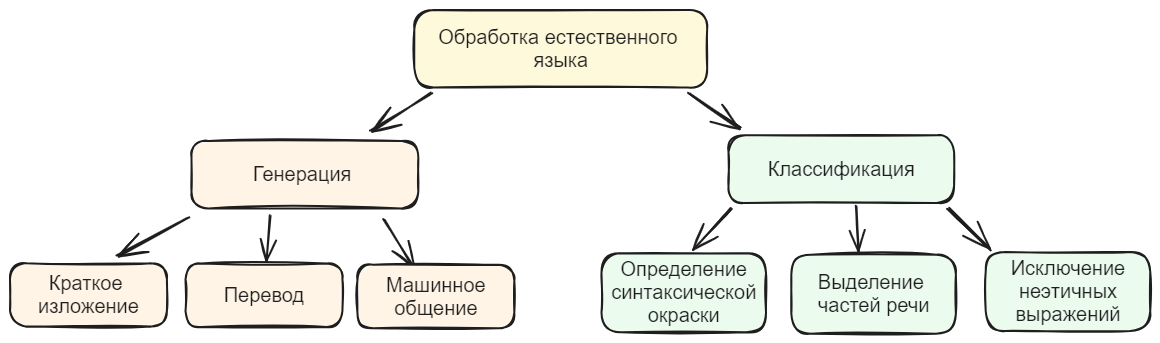
\includegraphics[width=0.5\textwidth]{assets/ml/nlp/taxonomy.excalidraw.png}
    \caption{Таксономия современных подходов обработки естественного языка}
    \label{llm_taxonomy}
\end{figure}

Формальные языки широко используются в математике, логике, лингвистике и компьютерных науках. 
В программировании, например, формальные языки включают языки программирования и описания данных, 
где синтаксис строго определён для обеспечения корректности и предсказуемости выполнения программ.

особенно важным для развития генеративного моделирования.
В областях обработки естественного языка стала популярна аналитическая форма механизма внимания \cite{vaswani2017attention},
приведшая к созданию больших лингвистических моделей \cite{radford2019language}, имеющих важное практическое применение.



\subsection{Оптимизация графа}

Задача оптимального транспорта (Optimal Transport)\cite{villani2009optimal} является одной из ключевых  
в области теории вероятностей и машинного обучения.
Она представляет собой проблему определения оптимального способа перемещения вероятностной массы из одной 
распределенной системы в другую с минимальными затратами или стоимостью. Формально задача состоит в составлении 
транспортного плана \( T: \mathcal{X} \rightarrow \mathcal{Y} \), 
который переводит распределение \( \mu \subset \mathcal{X}\) в распределение \( \nu \subset \mathcal{Y} \), минимизируя некоторую функцию стоимости. 
Функция стоимости $c: \mathcal{X} \times \mathcal{Y} \rightarrow \mathbb{R}$ обычно является мерой сходства между элементами из \( \mathcal{X} \) и \( \mathcal{Y} \), 
такой как квадрат расстояния. 

\textit{Определение} (Монже): \textbf{Оптимальный транспорт} по Монже вводится путем рассмотрения вероятностных 
распределений \( \mu \) и \( \nu \) на метрических пространствах \( \mathcal{X} \) и \( \mathcal{Y} \):
\begin{equation}
    \inf_{\gamma \in \Pi(\mu, \nu)} \int_{\mathcal{X} \times \mathcal{Y}} c(x,y) \, d\gamma(x,y),
\end{equation}
где \( \Pi(\mu, \nu) \) обозначает множество всех возможных совместных распределений 
\( \gamma \) на \( \mathcal{X} \times \mathcal{Y} \) с фиксированными маргинальными
распределениями \( \mu \) и \( \nu \), а \( c(x,y) \) — функция стоимости перевозки массы из \( x \) в \( y \).

\textit{Определение} (Канторович): \textbf{Оптимальный транспорт} по Канторовичу  вводится через потенциал $\phi$, 
который минимизирует функционал стоимости:
\begin{equation}
    \inf_{\phi} \left( \int_{\mathcal{X}} \phi(x) \, d\mu(x) + \int_{\mathcal{Y}} \psi(y) \, d\nu(y) \right),
\end{equation}
где \( \psi \) — обратная функция к \( \phi \). Таким образом, 
отображение \( T: \mathcal{X} \rightarrow \mathcal{Y} \) вытекает из градиента потенциала.

Заметим, что постановка Канторовича обобщает постановку Монже\ref{monge_vs_kantarovich}. В отличие от постановки Монже 
оптимальный транспорт по Канторовичу допускает распределение вероятностной массы в непрерывном случае.

\begin{figure}[h]
    \centering
    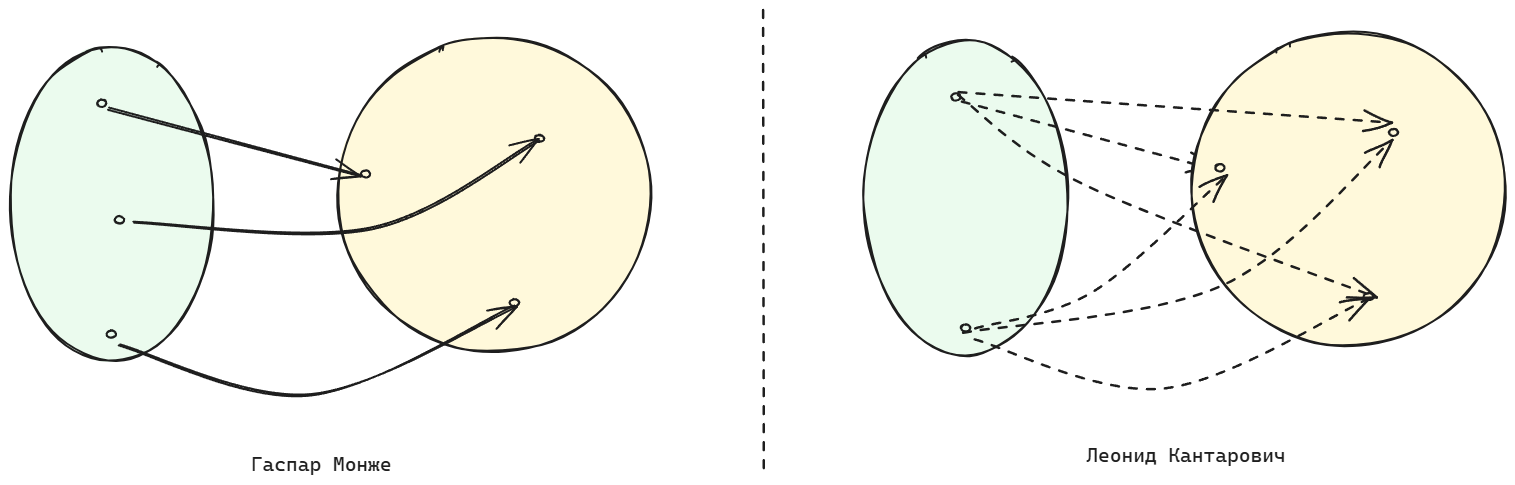
\includegraphics[width=0.7\textwidth]{assets/math/transport/optimal_transport.excalidraw.png}
    \caption{Различие в подходе по Монже и Кантаровичу. В постановке Канторовича задача релаксирует до 
    непрерывного распределения}
    \label{monge_vs_kantarovich}
\end{figure}

Итоговая стоимость оптимального транспортного плана называется метрикой Вассерштейна.

\textit{Определение:} Пусть \((X, d)\) --- метрическое пространство и \(P(X)\) --- множество всех вероятностных мер на \(X\). 
Для двух вероятностных мер \(\mu\) и \(\nu\) на \(X\) \textbf{метрика Вассерштейна} порядка \(p\), где \(p \geq 1\), определяется как:
\begin{equation}
    W_p(\mu, \nu) = \left( \inf_{\gamma \in \Gamma(\mu, \nu)} \int_{X \times X} d(x, y)^p \, d\gamma(x, y) \right)^{1/p},
\end{equation}
где \(\Gamma(\mu, \nu)\) — множество всех сопряжённых мер \(\gamma\) на \(X \times X\) с маргиналами \(\mu\) и \(\nu\).

Метрика имеет практическое применение для задач физики, биологии и машинного обучения, поскольку задает 
дифференцируемую разность между распределениями.

\textit{Определение:} \textbf{Метрическая производная} кривой $\rho_t,t \in [0,T]$ в вероятностном 
пространстве $\mathcal{P}_2(\mathbb{R}^N)$ запишется как:
\begin{equation}
    |\rho_t'| = \lim_{dt \rightarrow 0} \frac{\mathcal{W}_2(\rho_t, \rho_{t+dt})}{dt}
\end{equation}

Метод оптимального транспорта также активно применяется для анализа стохастических процессов. Базовой моделью, 
описывающей стохастическое движение с смещением, является процесс Ланжевена.

\textit{Определение:} Процесс Ланжевена называется случайнный процесс вида
\begin{equation}
    d X_t = - \nabla \Phi(x) dt + \sqrt{2 \beta^{-1}} d W_t,
\end{equation}
где $\Phi(X)$ --- потенциал задающий снос частицы, $\beta$ - масштаб блуждания и  $d W_t$ - процесс Винера.

\begin{figure}[h]
    \centering
    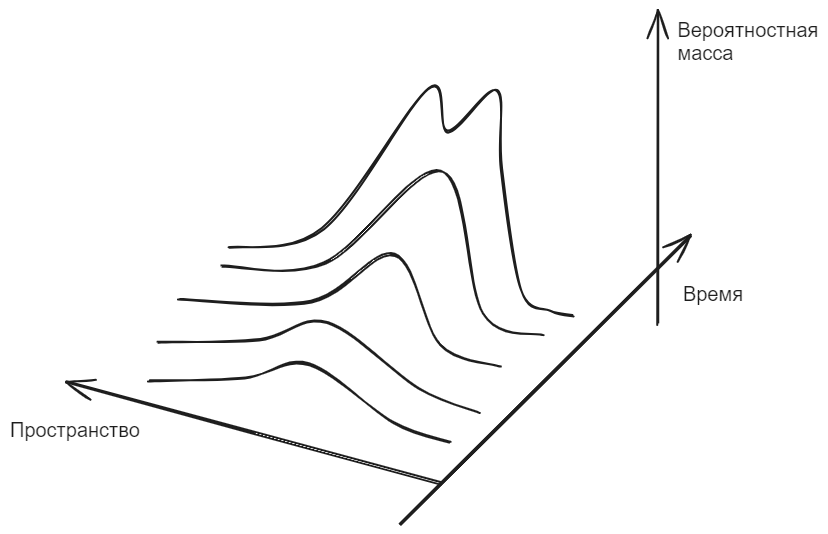
\includegraphics[width=0.5\textwidth]{assets/math/transport/fokker-plank.excalidraw.png}
    \caption{Эволюция вероятностной массы в уравнение Ланжевена}
    \label{opt_transport}
\end{figure}

Стохастическое усреднение процесса Ланжевена можно описать с помощью уравнения Колмогорова-Фоккера-Планка, 
задающего эволюцию вероятностной массы в дифференциальной форме  $\rho_t(x)$:
\begin{equation}
    \frac{\partial \rho_t}{\partial t} = \text{div}(\nabla \Phi(x) \rho_t) + \beta^{-1} \Delta \rho_t.
\end{equation}

Для естественной работы в энергетических постановках водится функционал, задающий коэффициента сноса с потенциалом $\Phi$.
Таким образом, исходное уравнение можно переписать в вариационной постановке \ref{variation_fp}.

\textit{Определение:} \textbf{Функционал Фоккера-Планка} для распределения $\rho$ записывается как: 
\begin{equation}
    \mathcal{F}_{FP}(\rho) = \int  \Phi(x) d\rho(x) + \beta^{-1} \int \log \rho(x) d \rho(x).
\end{equation}
\begin{figure}[h]
    \centering
    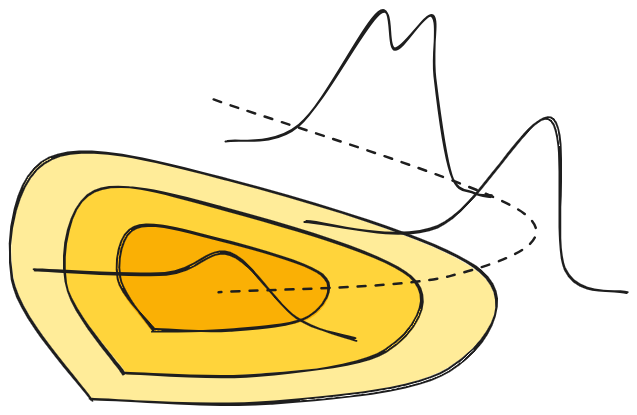
\includegraphics[width=0.5\textwidth]{assets/math/transport/functional.excalidraw.png}
    \caption{Визуализация постановки уравнения Фоккера-Планка в вариационной форме}
    \label{variation_fp}
\end{figure}
Научная группа Йордана-Кинана-Отто в работе \cite{jordan1998variational} показала, что маргинальные вероятностные
меры процесса Ланжевена подчиняются уравнению градиентного потока Вассерштейна относительно функционала Фоккера-Планка.

\textit{Определение:}  \textbf{Схема Йордана-Кинана-Отто} задает правило обновления уравнения вероятности в виде
минимизации функционала энергии и расстояния:
\begin{equation}
    \rho^{n+1} = \underset{\rho}{\operatorname{argmin}} \left( \frac{1}{2\tau} W_2^2(\rho, \rho^n) + \mathcal{F}(\rho) \right),
\end{equation}
где:\begin{itemize}
    \item \(\tau > 0\) --- шаг по времени;
    \item \(W_2(\rho, \rho^n)\) --- метрика Вассерштейна 2-го порядка между плотностями \(\rho\) и \(\rho^n\);
    \item  \(\mathcal{F}(\rho)\) --- функционал свободной энергии, который может включать в себя энтропийный член и 
    потенциальную энергию системы.
\end{itemize}
Функционал свободной энергии\(\mathcal{F}(\rho)\) задается в виде:
\begin{equation}
    \mathcal{F}(\rho) = \int_V f(\rho(x)) \, dx + \int_V V(x) \rho(x) \, dx,
\end{equation}
где \(f(\rho)\) — внутренний энергетический член, зависящий от плотности, а \(V(x)\) — внешний потенциал.




\chapter{Заключение}
Анализ естественного языка это межпредметная дисциплина.

\begin{figure}[h]
    \centering
    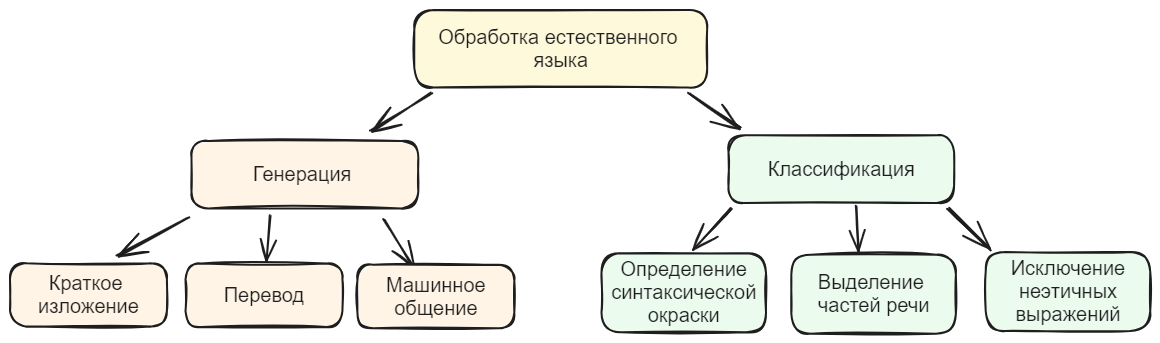
\includegraphics[width=0.5\textwidth]{assets/ml/nlp/taxonomy.excalidraw.png}
    \caption{Таксономия современных подходов обработки естественного языка}
    \label{llm_taxonomy}
\end{figure}

Формальные языки широко используются в математике, логике, лингвистике и компьютерных науках. 
В программировании, например, формальные языки включают языки программирования и описания данных, 
где синтаксис строго определён для обеспечения корректности и предсказуемости выполнения программ.

особенно важным для развития генеративного моделирования.
В областях обработки естественного языка стала популярна аналитическая форма механизма внимания \cite{vaswani2017attention},
приведшая к созданию больших лингвистических моделей \cite{radford2019language}, имеющих важное практическое применение.



\subsection{Оптимизация графа}

Задача оптимального транспорта (Optimal Transport)\cite{villani2009optimal} является одной из ключевых  
в области теории вероятностей и машинного обучения.
Она представляет собой проблему определения оптимального способа перемещения вероятностной массы из одной 
распределенной системы в другую с минимальными затратами или стоимостью. Формально задача состоит в составлении 
транспортного плана \( T: \mathcal{X} \rightarrow \mathcal{Y} \), 
который переводит распределение \( \mu \subset \mathcal{X}\) в распределение \( \nu \subset \mathcal{Y} \), минимизируя некоторую функцию стоимости. 
Функция стоимости $c: \mathcal{X} \times \mathcal{Y} \rightarrow \mathbb{R}$ обычно является мерой сходства между элементами из \( \mathcal{X} \) и \( \mathcal{Y} \), 
такой как квадрат расстояния. 

\textit{Определение} (Монже): \textbf{Оптимальный транспорт} по Монже вводится путем рассмотрения вероятностных 
распределений \( \mu \) и \( \nu \) на метрических пространствах \( \mathcal{X} \) и \( \mathcal{Y} \):
\begin{equation}
    \inf_{\gamma \in \Pi(\mu, \nu)} \int_{\mathcal{X} \times \mathcal{Y}} c(x,y) \, d\gamma(x,y),
\end{equation}
где \( \Pi(\mu, \nu) \) обозначает множество всех возможных совместных распределений 
\( \gamma \) на \( \mathcal{X} \times \mathcal{Y} \) с фиксированными маргинальными
распределениями \( \mu \) и \( \nu \), а \( c(x,y) \) — функция стоимости перевозки массы из \( x \) в \( y \).

\textit{Определение} (Канторович): \textbf{Оптимальный транспорт} по Канторовичу  вводится через потенциал $\phi$, 
который минимизирует функционал стоимости:
\begin{equation}
    \inf_{\phi} \left( \int_{\mathcal{X}} \phi(x) \, d\mu(x) + \int_{\mathcal{Y}} \psi(y) \, d\nu(y) \right),
\end{equation}
где \( \psi \) — обратная функция к \( \phi \). Таким образом, 
отображение \( T: \mathcal{X} \rightarrow \mathcal{Y} \) вытекает из градиента потенциала.

Заметим, что постановка Канторовича обобщает постановку Монже\ref{monge_vs_kantarovich}. В отличие от постановки Монже 
оптимальный транспорт по Канторовичу допускает распределение вероятностной массы в непрерывном случае.

\begin{figure}[h]
    \centering
    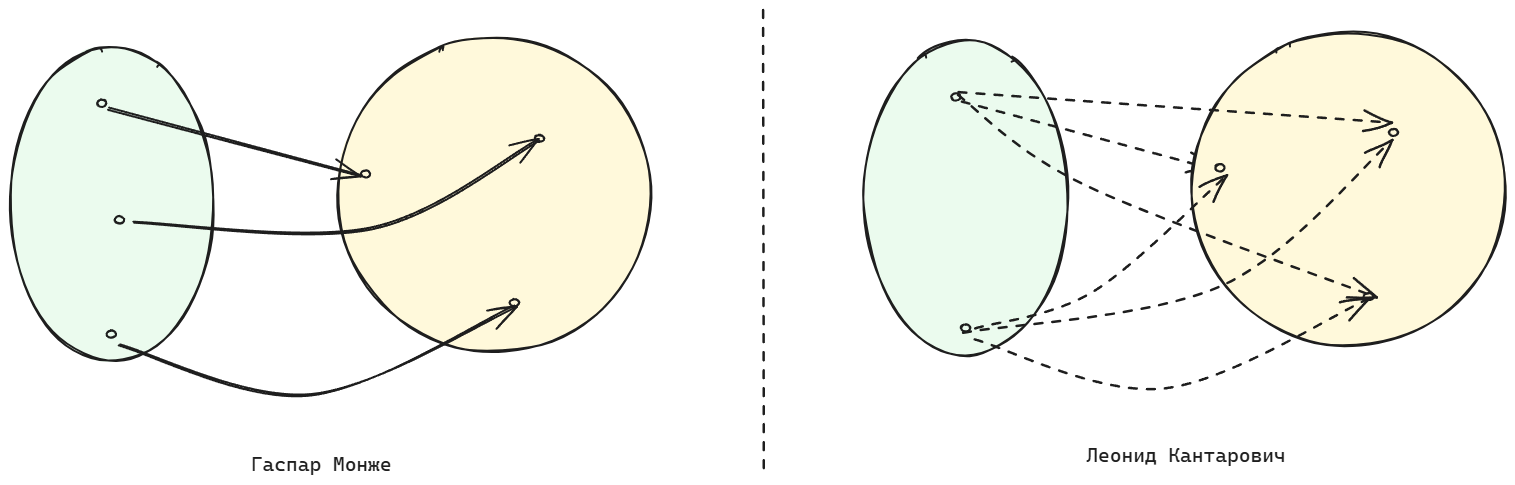
\includegraphics[width=0.7\textwidth]{assets/math/transport/optimal_transport.excalidraw.png}
    \caption{Различие в подходе по Монже и Кантаровичу. В постановке Канторовича задача релаксирует до 
    непрерывного распределения}
    \label{monge_vs_kantarovich}
\end{figure}

Итоговая стоимость оптимального транспортного плана называется метрикой Вассерштейна.

\textit{Определение:} Пусть \((X, d)\) --- метрическое пространство и \(P(X)\) --- множество всех вероятностных мер на \(X\). 
Для двух вероятностных мер \(\mu\) и \(\nu\) на \(X\) \textbf{метрика Вассерштейна} порядка \(p\), где \(p \geq 1\), определяется как:
\begin{equation}
    W_p(\mu, \nu) = \left( \inf_{\gamma \in \Gamma(\mu, \nu)} \int_{X \times X} d(x, y)^p \, d\gamma(x, y) \right)^{1/p},
\end{equation}
где \(\Gamma(\mu, \nu)\) — множество всех сопряжённых мер \(\gamma\) на \(X \times X\) с маргиналами \(\mu\) и \(\nu\).

Метрика имеет практическое применение для задач физики, биологии и машинного обучения, поскольку задает 
дифференцируемую разность между распределениями.

\textit{Определение:} \textbf{Метрическая производная} кривой $\rho_t,t \in [0,T]$ в вероятностном 
пространстве $\mathcal{P}_2(\mathbb{R}^N)$ запишется как:
\begin{equation}
    |\rho_t'| = \lim_{dt \rightarrow 0} \frac{\mathcal{W}_2(\rho_t, \rho_{t+dt})}{dt}
\end{equation}

Метод оптимального транспорта также активно применяется для анализа стохастических процессов. Базовой моделью, 
описывающей стохастическое движение с смещением, является процесс Ланжевена.

\textit{Определение:} Процесс Ланжевена называется случайнный процесс вида
\begin{equation}
    d X_t = - \nabla \Phi(x) dt + \sqrt{2 \beta^{-1}} d W_t,
\end{equation}
где $\Phi(X)$ --- потенциал задающий снос частицы, $\beta$ - масштаб блуждания и  $d W_t$ - процесс Винера.

\begin{figure}[h]
    \centering
    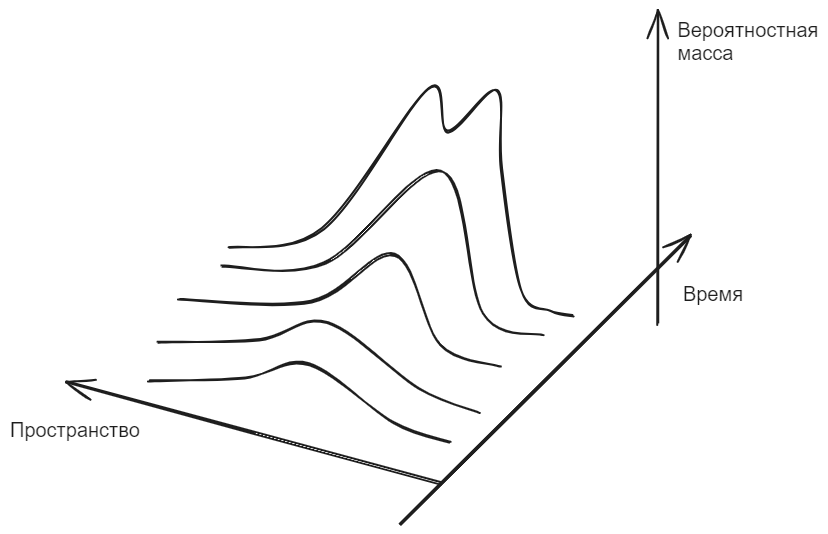
\includegraphics[width=0.5\textwidth]{assets/math/transport/fokker-plank.excalidraw.png}
    \caption{Эволюция вероятностной массы в уравнение Ланжевена}
    \label{opt_transport}
\end{figure}

Стохастическое усреднение процесса Ланжевена можно описать с помощью уравнения Колмогорова-Фоккера-Планка, 
задающего эволюцию вероятностной массы в дифференциальной форме  $\rho_t(x)$:
\begin{equation}
    \frac{\partial \rho_t}{\partial t} = \text{div}(\nabla \Phi(x) \rho_t) + \beta^{-1} \Delta \rho_t.
\end{equation}

Для естественной работы в энергетических постановках водится функционал, задающий коэффициента сноса с потенциалом $\Phi$.
Таким образом, исходное уравнение можно переписать в вариационной постановке \ref{variation_fp}.

\textit{Определение:} \textbf{Функционал Фоккера-Планка} для распределения $\rho$ записывается как: 
\begin{equation}
    \mathcal{F}_{FP}(\rho) = \int  \Phi(x) d\rho(x) + \beta^{-1} \int \log \rho(x) d \rho(x).
\end{equation}
\begin{figure}[h]
    \centering
    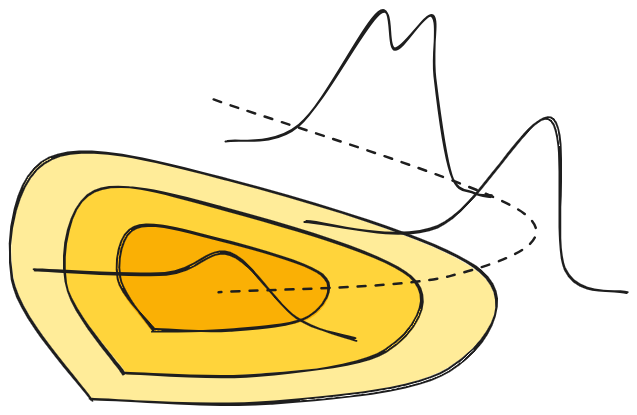
\includegraphics[width=0.5\textwidth]{assets/math/transport/functional.excalidraw.png}
    \caption{Визуализация постановки уравнения Фоккера-Планка в вариационной форме}
    \label{variation_fp}
\end{figure}
Научная группа Йордана-Кинана-Отто в работе \cite{jordan1998variational} показала, что маргинальные вероятностные
меры процесса Ланжевена подчиняются уравнению градиентного потока Вассерштейна относительно функционала Фоккера-Планка.

\textit{Определение:}  \textbf{Схема Йордана-Кинана-Отто} задает правило обновления уравнения вероятности в виде
минимизации функционала энергии и расстояния:
\begin{equation}
    \rho^{n+1} = \underset{\rho}{\operatorname{argmin}} \left( \frac{1}{2\tau} W_2^2(\rho, \rho^n) + \mathcal{F}(\rho) \right),
\end{equation}
где:\begin{itemize}
    \item \(\tau > 0\) --- шаг по времени;
    \item \(W_2(\rho, \rho^n)\) --- метрика Вассерштейна 2-го порядка между плотностями \(\rho\) и \(\rho^n\);
    \item  \(\mathcal{F}(\rho)\) --- функционал свободной энергии, который может включать в себя энтропийный член и 
    потенциальную энергию системы.
\end{itemize}
Функционал свободной энергии\(\mathcal{F}(\rho)\) задается в виде:
\begin{equation}
    \mathcal{F}(\rho) = \int_V f(\rho(x)) \, dx + \int_V V(x) \rho(x) \, dx,
\end{equation}
где \(f(\rho)\) — внутренний энергетический член, зависящий от плотности, а \(V(x)\) — внешний потенциал.





\printbib

Анализ естественного языка это межпредметная дисциплина.

\begin{figure}[h]
    \centering
    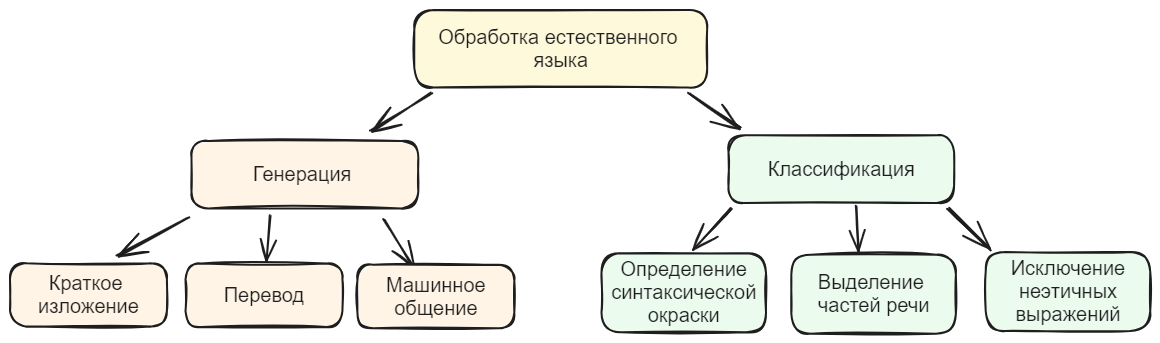
\includegraphics[width=0.5\textwidth]{assets/ml/nlp/taxonomy.excalidraw.png}
    \caption{Таксономия современных подходов обработки естественного языка}
    \label{llm_taxonomy}
\end{figure}

Формальные языки широко используются в математике, логике, лингвистике и компьютерных науках. 
В программировании, например, формальные языки включают языки программирования и описания данных, 
где синтаксис строго определён для обеспечения корректности и предсказуемости выполнения программ.

особенно важным для развития генеративного моделирования.
В областях обработки естественного языка стала популярна аналитическая форма механизма внимания \cite{vaswani2017attention},
приведшая к созданию больших лингвистических моделей \cite{radford2019language}, имеющих важное практическое применение.



\subsection{Оптимизация графа}

Задача оптимального транспорта (Optimal Transport)\cite{villani2009optimal} является одной из ключевых  
в области теории вероятностей и машинного обучения.
Она представляет собой проблему определения оптимального способа перемещения вероятностной массы из одной 
распределенной системы в другую с минимальными затратами или стоимостью. Формально задача состоит в составлении 
транспортного плана \( T: \mathcal{X} \rightarrow \mathcal{Y} \), 
который переводит распределение \( \mu \subset \mathcal{X}\) в распределение \( \nu \subset \mathcal{Y} \), минимизируя некоторую функцию стоимости. 
Функция стоимости $c: \mathcal{X} \times \mathcal{Y} \rightarrow \mathbb{R}$ обычно является мерой сходства между элементами из \( \mathcal{X} \) и \( \mathcal{Y} \), 
такой как квадрат расстояния. 

\textit{Определение} (Монже): \textbf{Оптимальный транспорт} по Монже вводится путем рассмотрения вероятностных 
распределений \( \mu \) и \( \nu \) на метрических пространствах \( \mathcal{X} \) и \( \mathcal{Y} \):
\begin{equation}
    \inf_{\gamma \in \Pi(\mu, \nu)} \int_{\mathcal{X} \times \mathcal{Y}} c(x,y) \, d\gamma(x,y),
\end{equation}
где \( \Pi(\mu, \nu) \) обозначает множество всех возможных совместных распределений 
\( \gamma \) на \( \mathcal{X} \times \mathcal{Y} \) с фиксированными маргинальными
распределениями \( \mu \) и \( \nu \), а \( c(x,y) \) — функция стоимости перевозки массы из \( x \) в \( y \).

\textit{Определение} (Канторович): \textbf{Оптимальный транспорт} по Канторовичу  вводится через потенциал $\phi$, 
который минимизирует функционал стоимости:
\begin{equation}
    \inf_{\phi} \left( \int_{\mathcal{X}} \phi(x) \, d\mu(x) + \int_{\mathcal{Y}} \psi(y) \, d\nu(y) \right),
\end{equation}
где \( \psi \) — обратная функция к \( \phi \). Таким образом, 
отображение \( T: \mathcal{X} \rightarrow \mathcal{Y} \) вытекает из градиента потенциала.

Заметим, что постановка Канторовича обобщает постановку Монже\ref{monge_vs_kantarovich}. В отличие от постановки Монже 
оптимальный транспорт по Канторовичу допускает распределение вероятностной массы в непрерывном случае.

\begin{figure}[h]
    \centering
    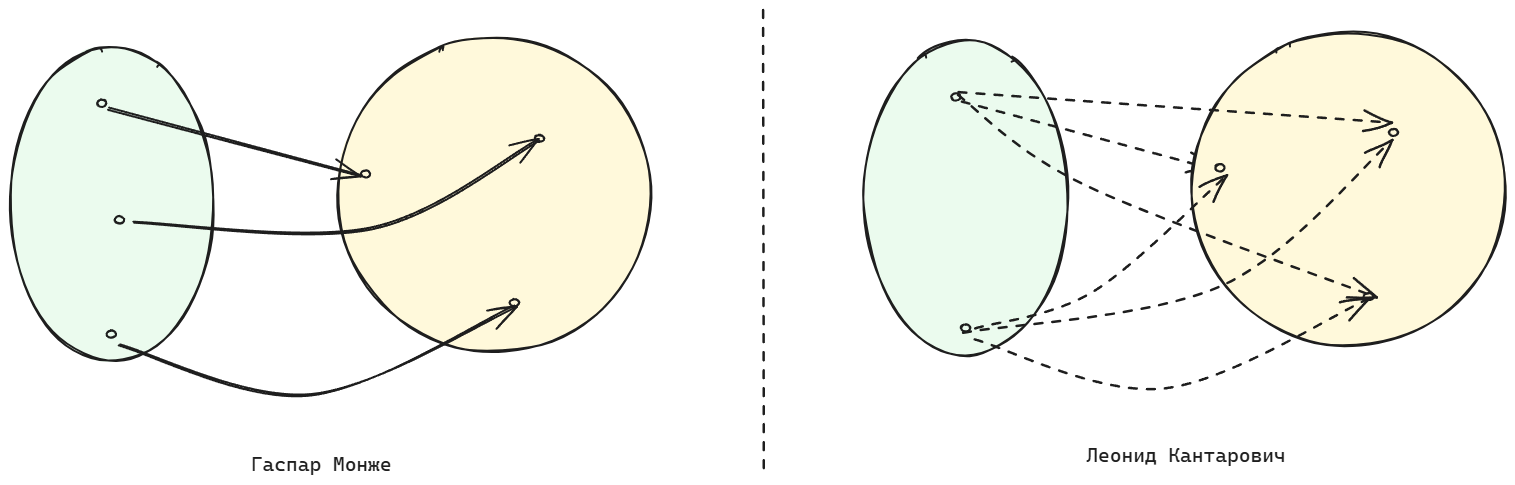
\includegraphics[width=0.7\textwidth]{assets/math/transport/optimal_transport.excalidraw.png}
    \caption{Различие в подходе по Монже и Кантаровичу. В постановке Канторовича задача релаксирует до 
    непрерывного распределения}
    \label{monge_vs_kantarovich}
\end{figure}

Итоговая стоимость оптимального транспортного плана называется метрикой Вассерштейна.

\textit{Определение:} Пусть \((X, d)\) --- метрическое пространство и \(P(X)\) --- множество всех вероятностных мер на \(X\). 
Для двух вероятностных мер \(\mu\) и \(\nu\) на \(X\) \textbf{метрика Вассерштейна} порядка \(p\), где \(p \geq 1\), определяется как:
\begin{equation}
    W_p(\mu, \nu) = \left( \inf_{\gamma \in \Gamma(\mu, \nu)} \int_{X \times X} d(x, y)^p \, d\gamma(x, y) \right)^{1/p},
\end{equation}
где \(\Gamma(\mu, \nu)\) — множество всех сопряжённых мер \(\gamma\) на \(X \times X\) с маргиналами \(\mu\) и \(\nu\).

Метрика имеет практическое применение для задач физики, биологии и машинного обучения, поскольку задает 
дифференцируемую разность между распределениями.

\textit{Определение:} \textbf{Метрическая производная} кривой $\rho_t,t \in [0,T]$ в вероятностном 
пространстве $\mathcal{P}_2(\mathbb{R}^N)$ запишется как:
\begin{equation}
    |\rho_t'| = \lim_{dt \rightarrow 0} \frac{\mathcal{W}_2(\rho_t, \rho_{t+dt})}{dt}
\end{equation}

Метод оптимального транспорта также активно применяется для анализа стохастических процессов. Базовой моделью, 
описывающей стохастическое движение с смещением, является процесс Ланжевена.

\textit{Определение:} Процесс Ланжевена называется случайнный процесс вида
\begin{equation}
    d X_t = - \nabla \Phi(x) dt + \sqrt{2 \beta^{-1}} d W_t,
\end{equation}
где $\Phi(X)$ --- потенциал задающий снос частицы, $\beta$ - масштаб блуждания и  $d W_t$ - процесс Винера.

\begin{figure}[h]
    \centering
    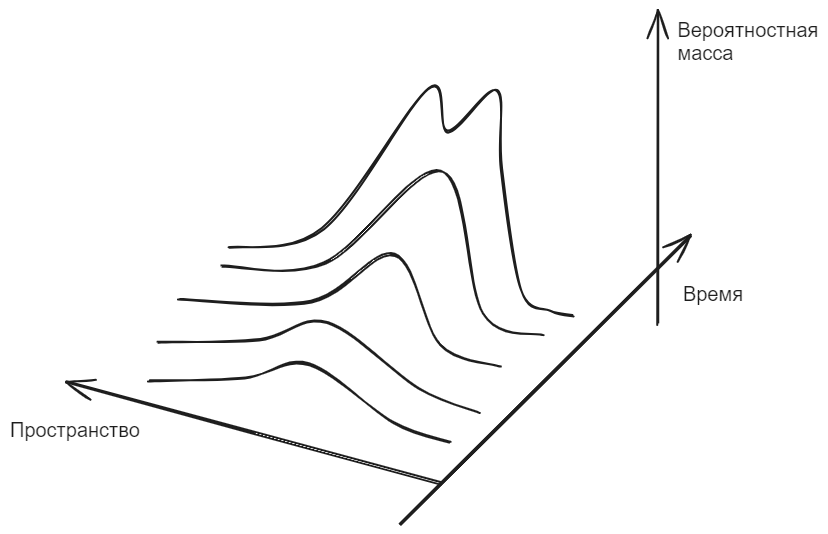
\includegraphics[width=0.5\textwidth]{assets/math/transport/fokker-plank.excalidraw.png}
    \caption{Эволюция вероятностной массы в уравнение Ланжевена}
    \label{opt_transport}
\end{figure}

Стохастическое усреднение процесса Ланжевена можно описать с помощью уравнения Колмогорова-Фоккера-Планка, 
задающего эволюцию вероятностной массы в дифференциальной форме  $\rho_t(x)$:
\begin{equation}
    \frac{\partial \rho_t}{\partial t} = \text{div}(\nabla \Phi(x) \rho_t) + \beta^{-1} \Delta \rho_t.
\end{equation}

Для естественной работы в энергетических постановках водится функционал, задающий коэффициента сноса с потенциалом $\Phi$.
Таким образом, исходное уравнение можно переписать в вариационной постановке \ref{variation_fp}.

\textit{Определение:} \textbf{Функционал Фоккера-Планка} для распределения $\rho$ записывается как: 
\begin{equation}
    \mathcal{F}_{FP}(\rho) = \int  \Phi(x) d\rho(x) + \beta^{-1} \int \log \rho(x) d \rho(x).
\end{equation}
\begin{figure}[h]
    \centering
    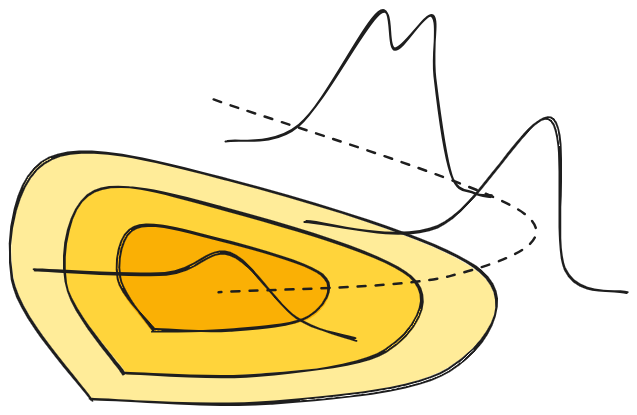
\includegraphics[width=0.5\textwidth]{assets/math/transport/functional.excalidraw.png}
    \caption{Визуализация постановки уравнения Фоккера-Планка в вариационной форме}
    \label{variation_fp}
\end{figure}
Научная группа Йордана-Кинана-Отто в работе \cite{jordan1998variational} показала, что маргинальные вероятностные
меры процесса Ланжевена подчиняются уравнению градиентного потока Вассерштейна относительно функционала Фоккера-Планка.

\textit{Определение:}  \textbf{Схема Йордана-Кинана-Отто} задает правило обновления уравнения вероятности в виде
минимизации функционала энергии и расстояния:
\begin{equation}
    \rho^{n+1} = \underset{\rho}{\operatorname{argmin}} \left( \frac{1}{2\tau} W_2^2(\rho, \rho^n) + \mathcal{F}(\rho) \right),
\end{equation}
где:\begin{itemize}
    \item \(\tau > 0\) --- шаг по времени;
    \item \(W_2(\rho, \rho^n)\) --- метрика Вассерштейна 2-го порядка между плотностями \(\rho\) и \(\rho^n\);
    \item  \(\mathcal{F}(\rho)\) --- функционал свободной энергии, который может включать в себя энтропийный член и 
    потенциальную энергию системы.
\end{itemize}
Функционал свободной энергии\(\mathcal{F}(\rho)\) задается в виде:
\begin{equation}
    \mathcal{F}(\rho) = \int_V f(\rho(x)) \, dx + \int_V V(x) \rho(x) \, dx,
\end{equation}
где \(f(\rho)\) — внутренний энергетический член, зависящий от плотности, а \(V(x)\) — внешний потенциал.





\end{document}